\documentclass{beamer}
\usetheme{Copenhagen}
\usepackage[utf8]{inputenc}
\usepackage{graphicx}
\graphicspath{ {images/} }
\usepackage{ amssymb }
\usepackage{ amsmath }

\title[Optimal Tip-To-Tip Efficiency: A Review] %optional
{Optimal Tip-to-Tip Efficiency: A Review}
\subtitle{A model for male audience stimulation}
\date[PPPT2019]{PowerPoint Party, October 2019}
\author[Bo]{M.~J.~Bo}
 
% \institute[VFU]
% {\inst{1}Atlassian}

\begin{document}
 
\frame{\titlepage}
 
\begin{frame}
\frametitle{Prior Art}

\bibliographystyle{ieeetr}
\bibliography{bib}
\end{frame}

\begin{frame}
    \begin{figure}
        \caption{Authors Chutgai, Gilfoyle, Dunn     \cite{BCDGH14}}
        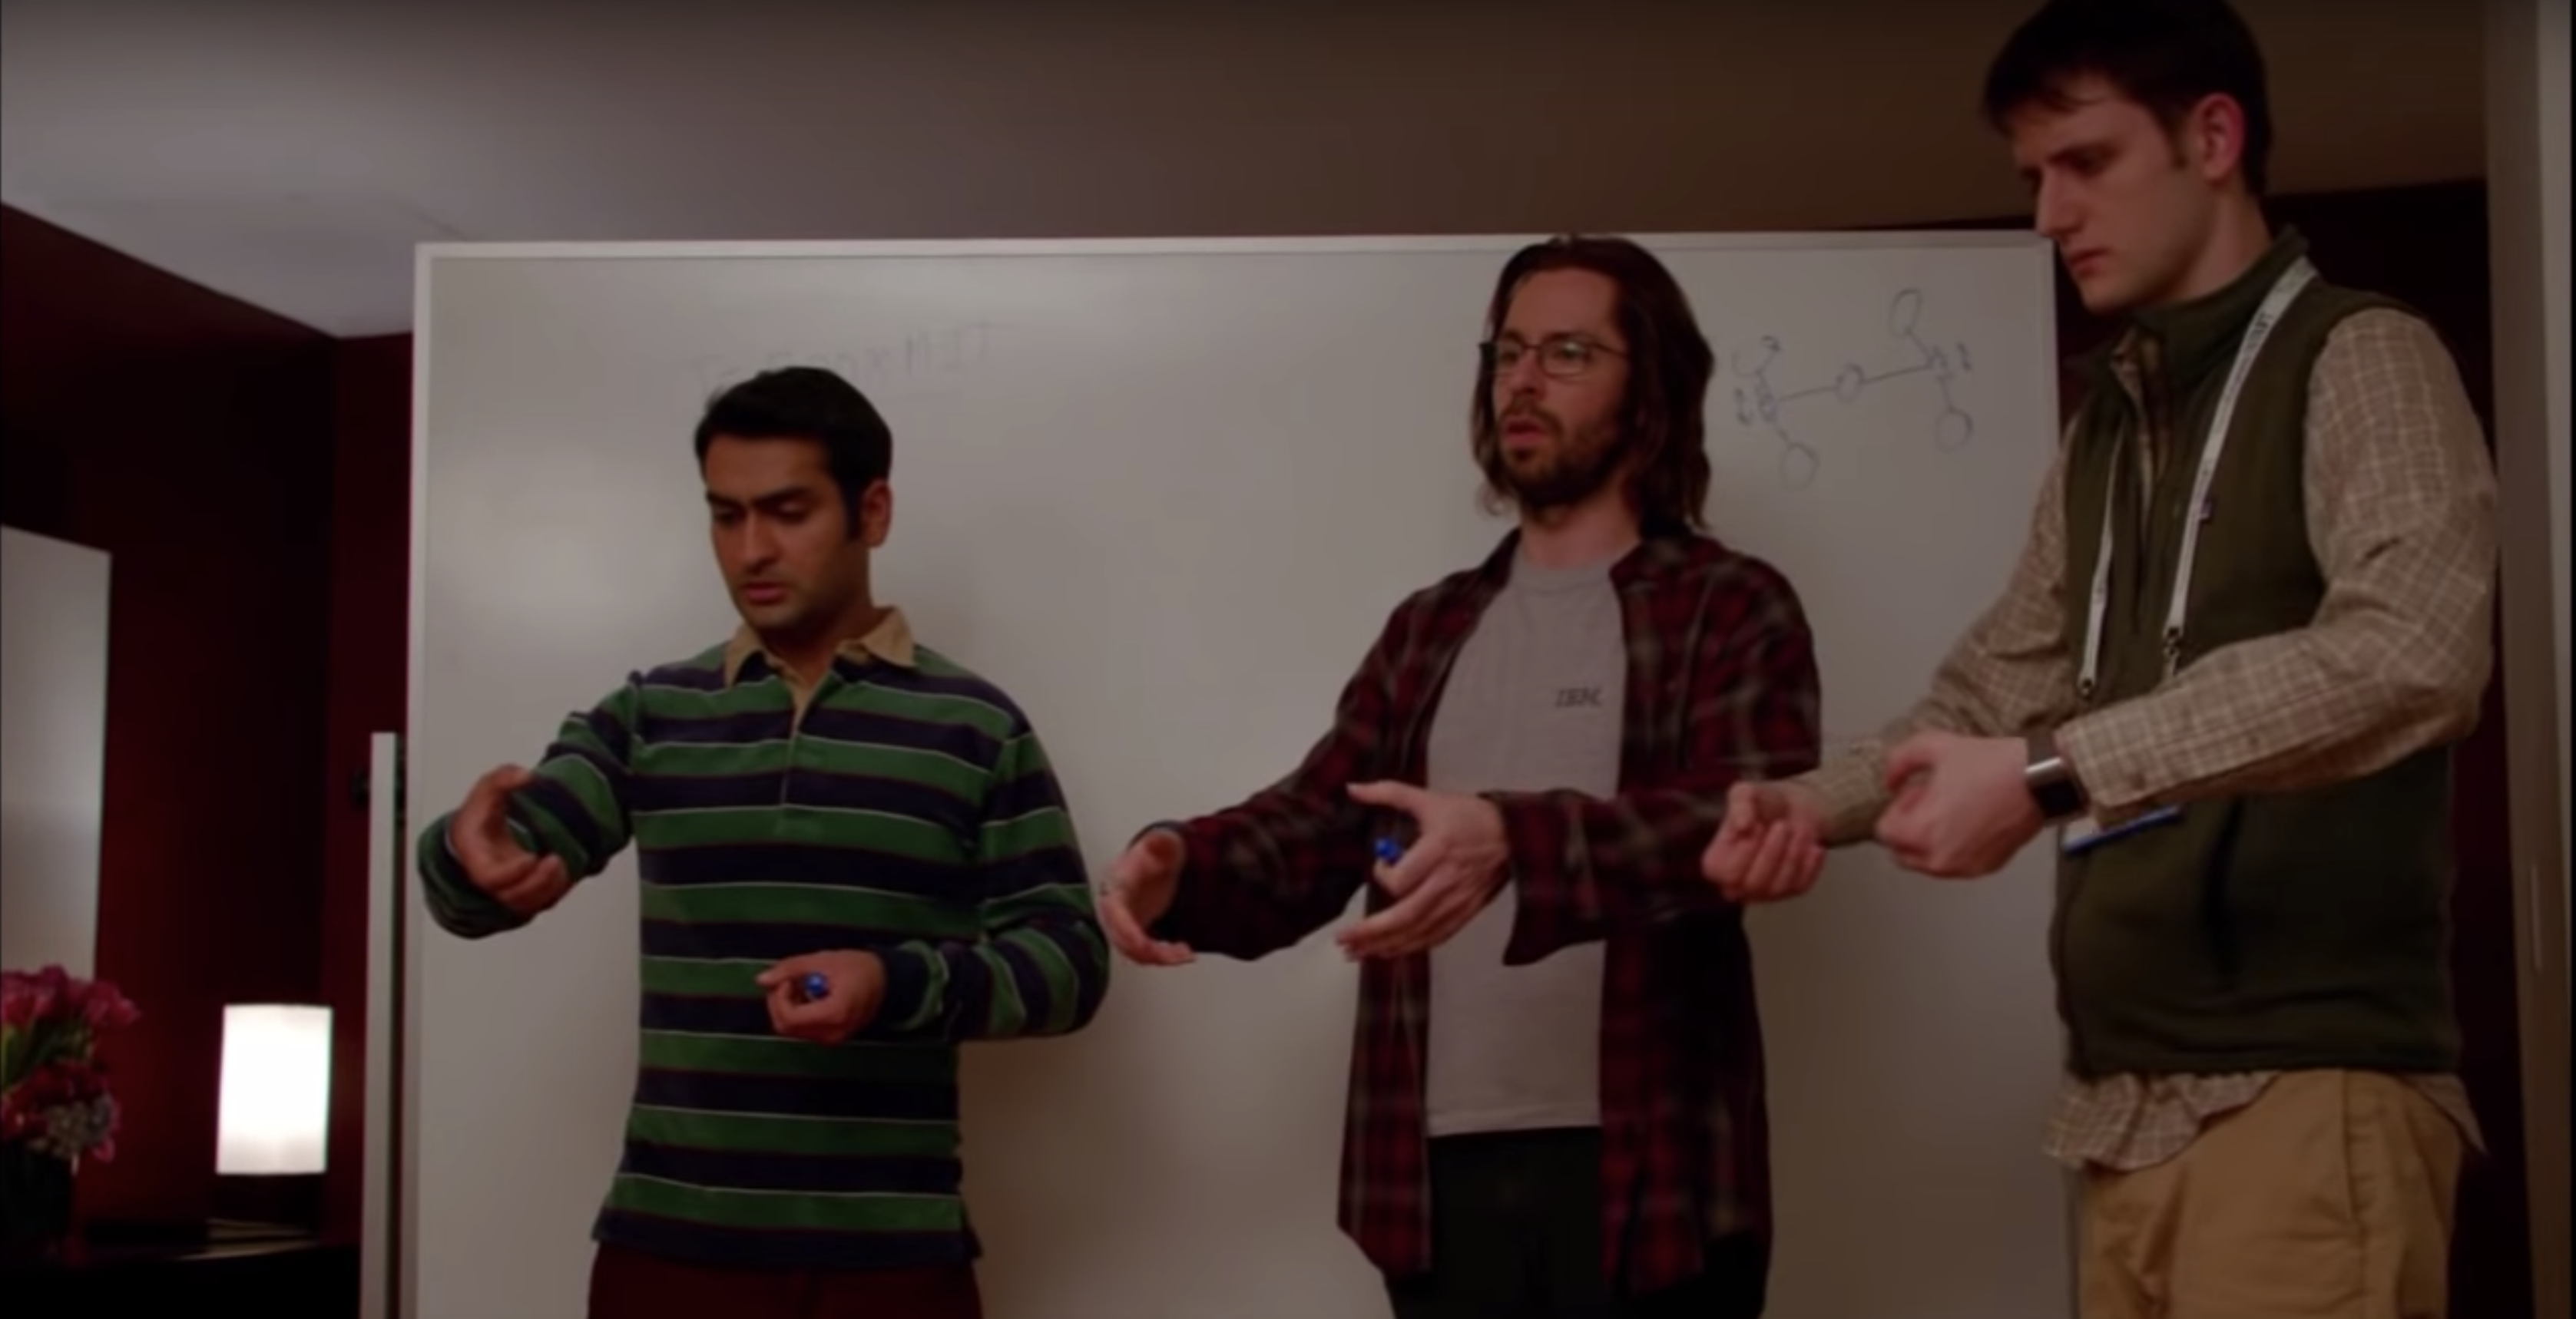
\includegraphics[width=9cm]{authors}
    \end{figure}
\end{frame}

\begin{frame}
    \begin{block}{Abstract}
        A probabilistic model is introduced for the problem of stimulating a large male audience. Double jerking is considered, in which two shafts may be stimulated with a single hand. Both tip-to-tip and shaft-to-shaft configurations of audience members are analyzed. We demonstrate that pre-sorting members of the audience according to both shaft girth and leg length allows for more efficient stimulation. Simulations establish steady rates of stimulation even as the variance of certain parameters is allowed to grow, whereas naive unsorted schemes have increasingly flaccid performance.
    \end{block}
\end{frame}

\begin{frame}
    \frametitle{Formulae}

    \begin{itemize}
        \item $D$ - girth\\
        \item $\Lambda$ - gratification threshold\\
        \item $f_s$ - shaft contact s.t. $f_s \in [0,1]$\\
        \item $f_t$ - time during a jerk action that that contact is maintained s.t. $f_t \in [0, 1]$\\
        \item $S(f)$ - spatial gratification function\\
        \item $T(f)$ - temporal gratification function\\
        \item $J$ - jerks
    \end{itemize}
\end{frame}

\begin{frame}
    \begin{itemize}
        \item $cum \triangleq JS(f_s)T(f_s)$ - cumulative gratification function\\
    \end{itemize}

    
    \begin{block}{Remark}
        \begin{itemize}
            \item Assume $T(f) = \sqrt{f}$ and $S(f) = \sqrt{f}$\\

            \item If $cum \geq \Lambda$, the audience member will invoke a climactic stimulation event\\
        \end{itemize}
    \end{block}


\end{frame}

\begin{frame}
    \frametitle{Multiple Simulation}

    \begin{enumerate}
        \item \textit{Tip-to-tip} (series jerking): two individuals stand facing one another, with their members touching tip-to-tip. A single hand moves across both shafts, treating them as one extra-long shaft.
        \item \textit{Shaft-to-shaft} (parallel jerking): Two individuals stand facing one another, with their members against one another lengthwise. A single hand wraps around both shafts, treating them as one extra-thick shaft.
    \end{enumerate}

    \begin{block}{Remark}
        We assume in the double jerk scenario that jerking \alert{must continue} until both members have exceeded their gratification threshold.
    \end{block}
\end{frame}

\begin{frame}
    \begin{figure}
        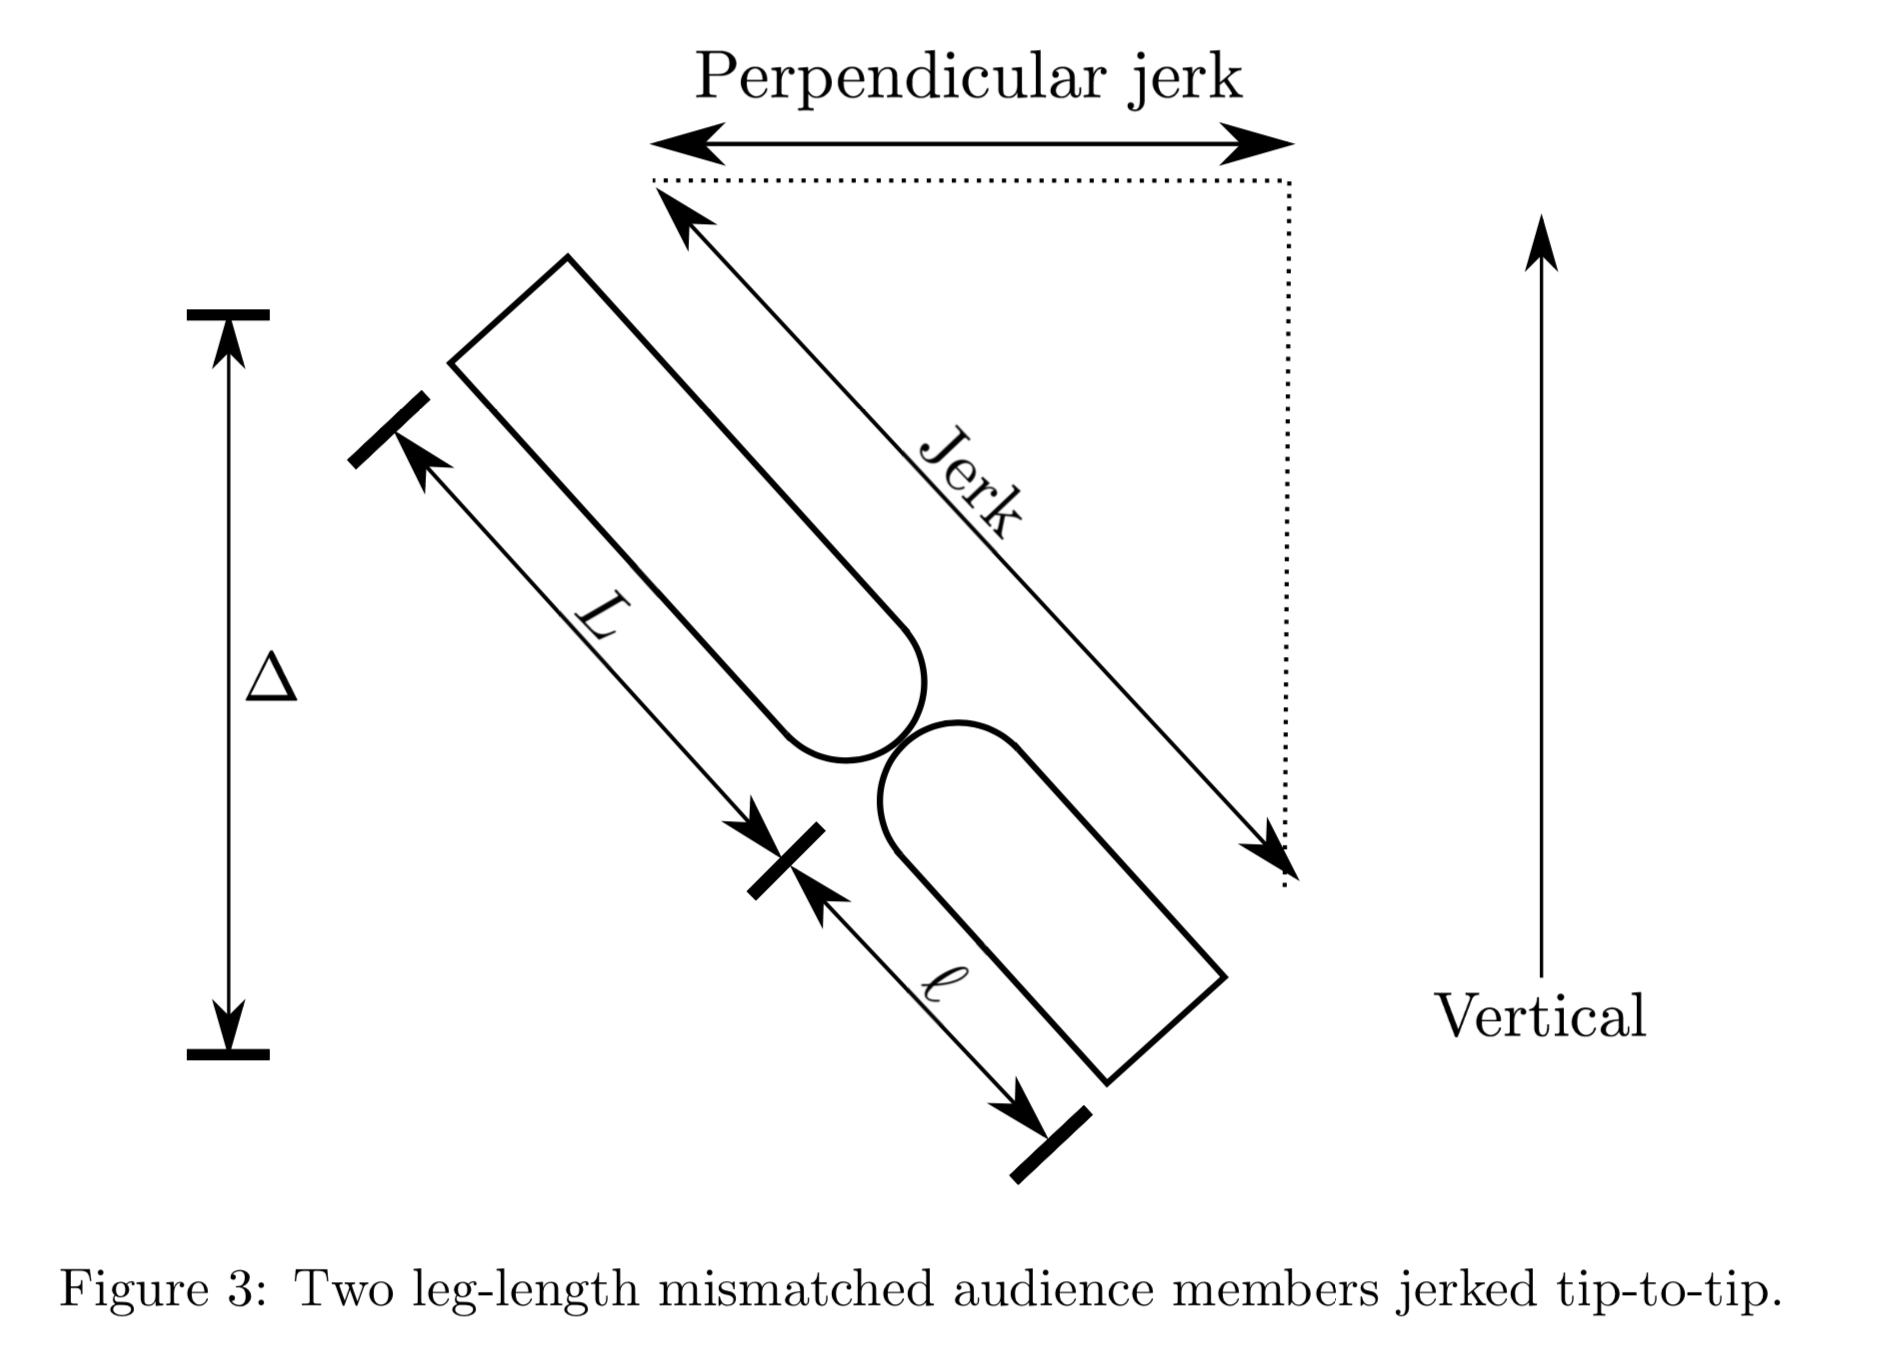
\includegraphics[width=9cm]{t2t}
    \end{figure}
\end{frame}

\begin{frame}
    \begin{figure}
        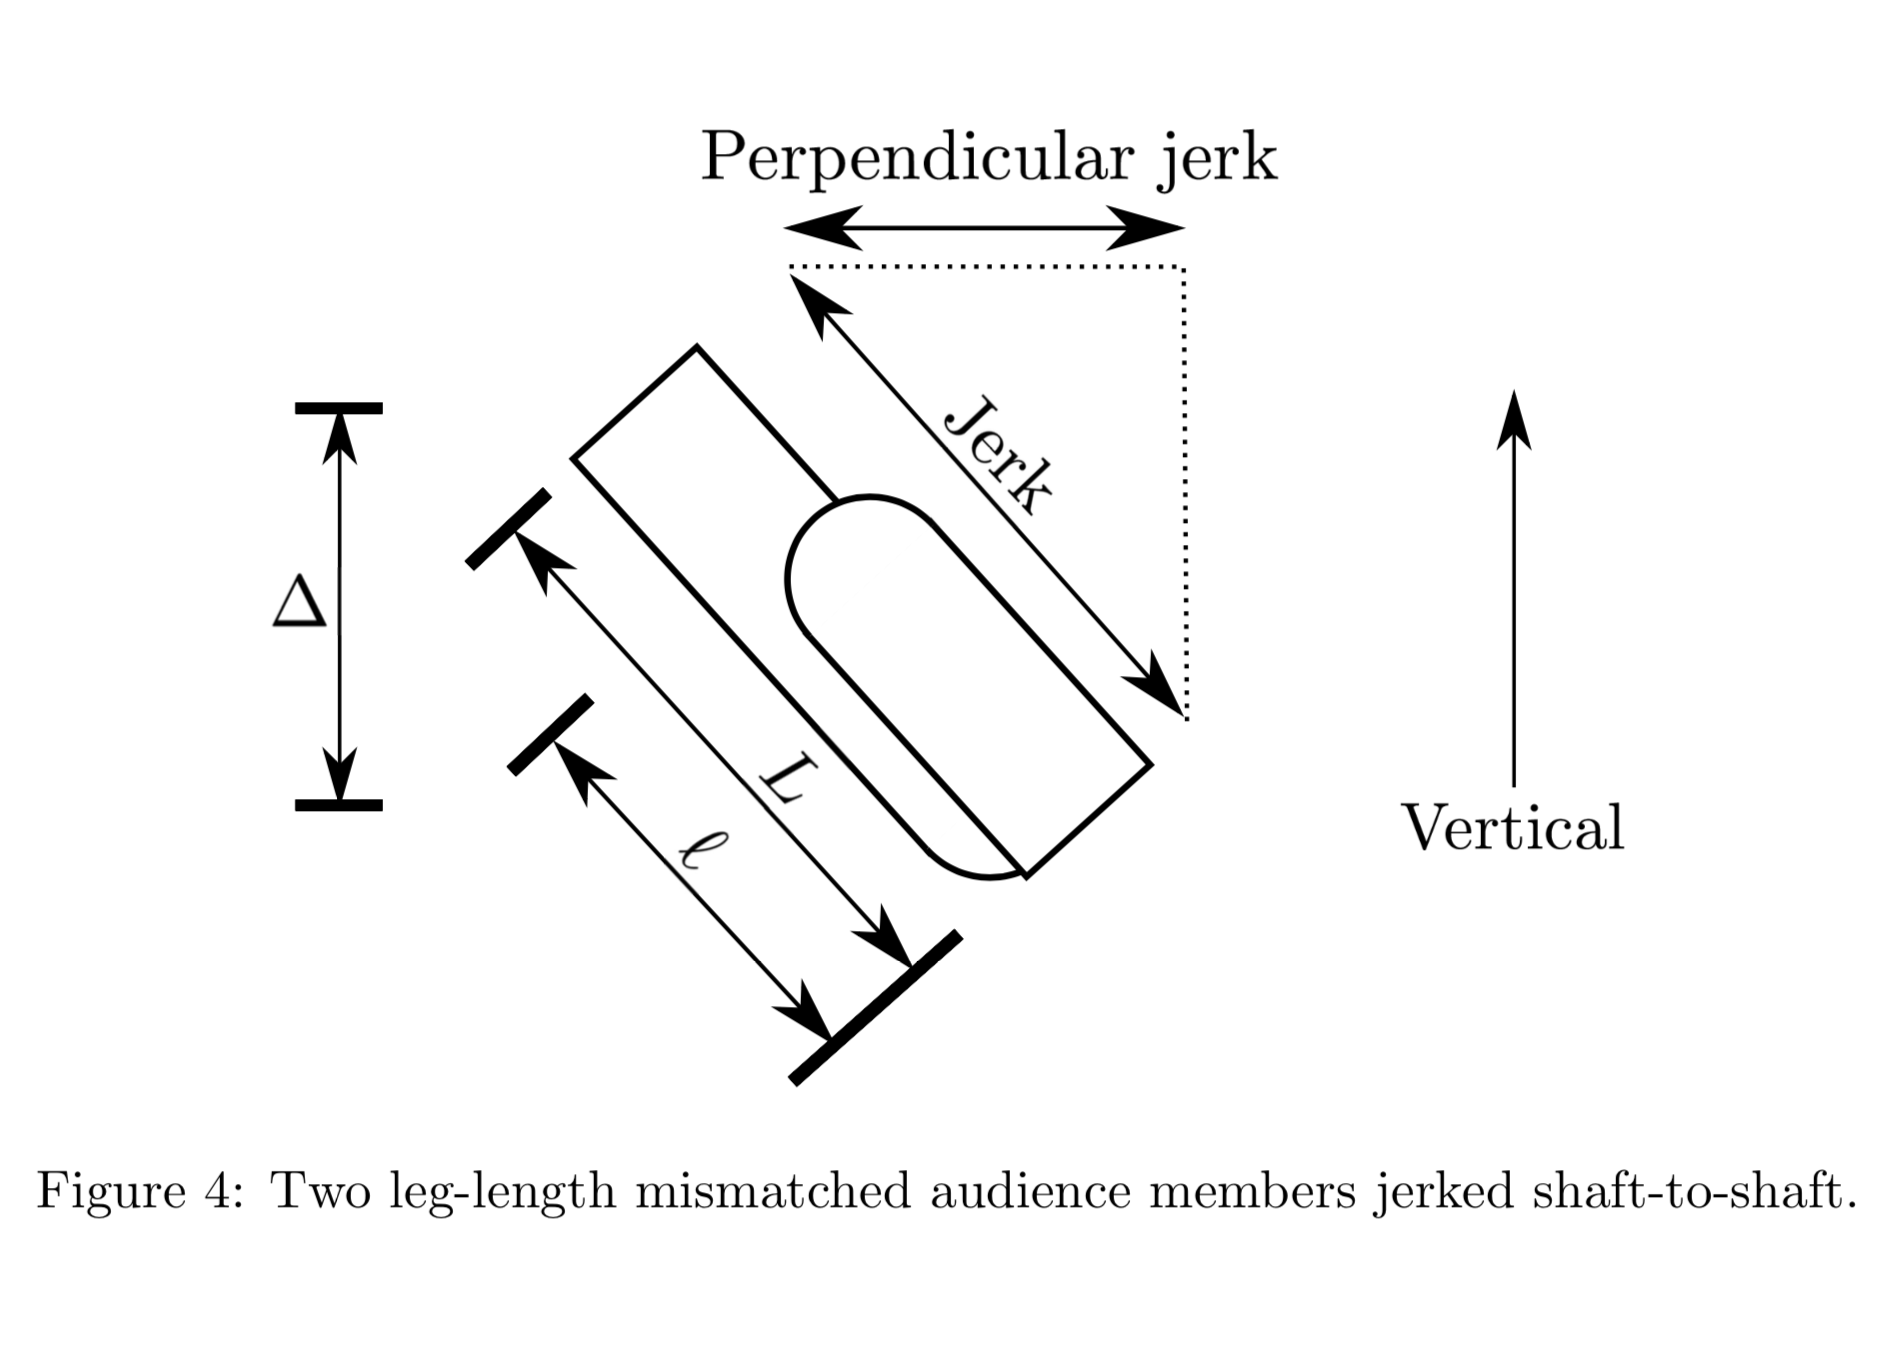
\includegraphics[width=9cm]{s2s}
    \end{figure}
\end{frame}

\begin{frame}
    If $\Delta \neq 0$ 

    \begin{enumerate}
        \item Ask the taller member to squat, in which case his gratification will be reduced from physical discomfort.
        \item Ask the shorter member to stand on a box. The humiliation will likely reduce his gratification as well.
        \item Attempt to double jerk vertically displaced shafts by angling the taller individual's shaft down and the shorter individual’s shaft up. The jerk direction will no longer be perpendicular to the individuals in this case (Figs. 3 and 4), so gratification will again be reduced.
    \end{enumerate}

\end{frame}

\begin{frame}

    Let $P_j$ be the gratification penalty, a reduced gratification-per-jerk.

    For the \textit{tip-to-tip} configuration (Fig. 3)

    \[
        P_j = S(f_s)T(f_t) \frac{\sqrt{(l + L)^2 - \Delta ^ 2}}{l + L}
    \]

    For the \textit{shaft-to-shaft} configuration (Fig. 4)

    \[
        P_j = S(f_s)T(f_t) \frac{\sqrt{(\max \{l, L\})^2 - \Delta ^ 2}}{\max \{l, L\}}
    \]

\end{frame}

\begin{frame}
    \begin{figure}
        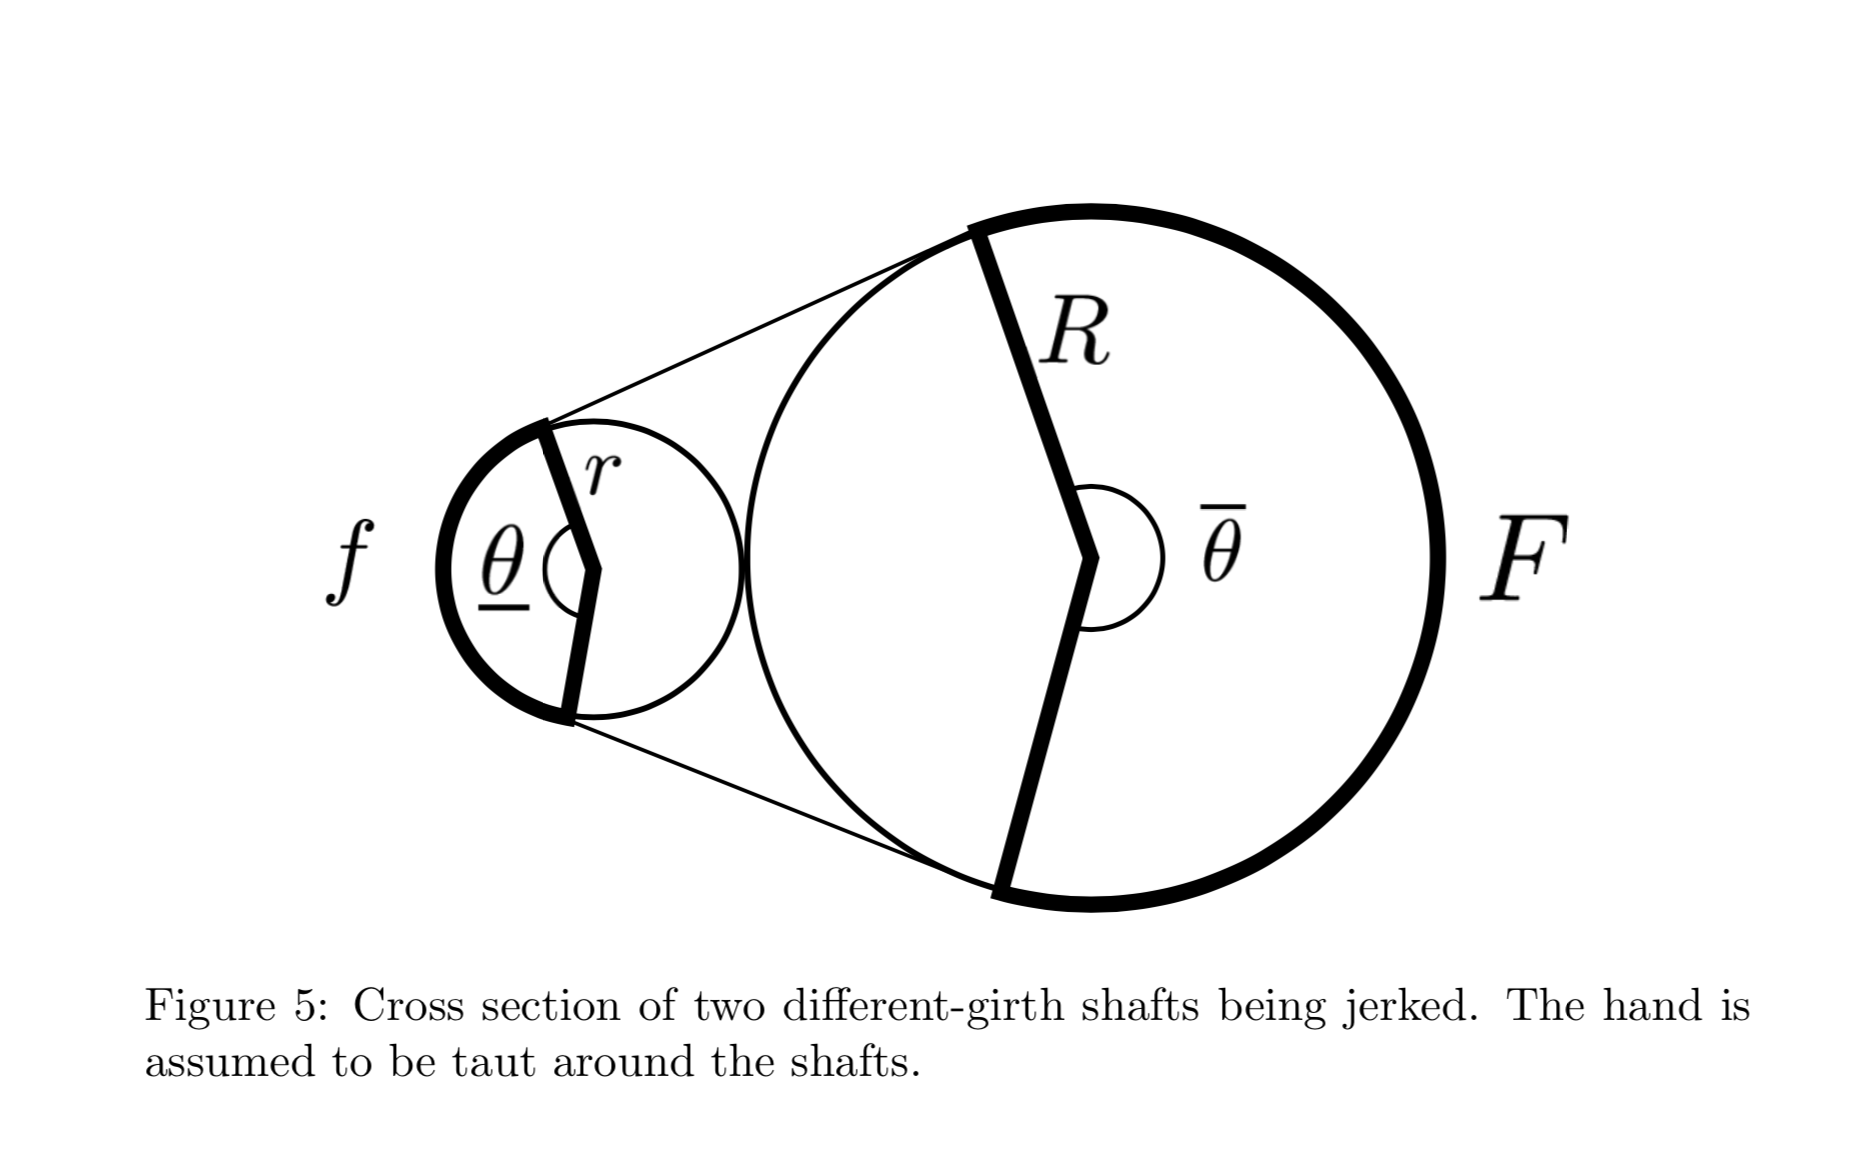
\includegraphics[width=9cm]{girth}
    \end{figure}
\end{frame}

\begin{frame}

    \[
        F = \frac{1}{2} + \frac{1}{\pi}\arcsin (\frac{R - r}{R + r})
    \]

    \[
        f = \frac{1}{2} - \frac{1}{\pi}\arcsin (\frac{R - r}{R + r})
    \]

\end{frame}

\begin{frame}
The suggested tip-to-tip scheme involves the following steps:
    \begin{enumerate}
        \item Sort the audience into bins corresponding to each leg length, at the resolution of a centimeter.
        \item Sort the members in each bin based on shaft length.
        \item Double jerk adjacent individuals from the same bin with each hand, tip-to-tip.
    \end{enumerate}
\end{frame}


\begin{frame}
    \begin{figure}
        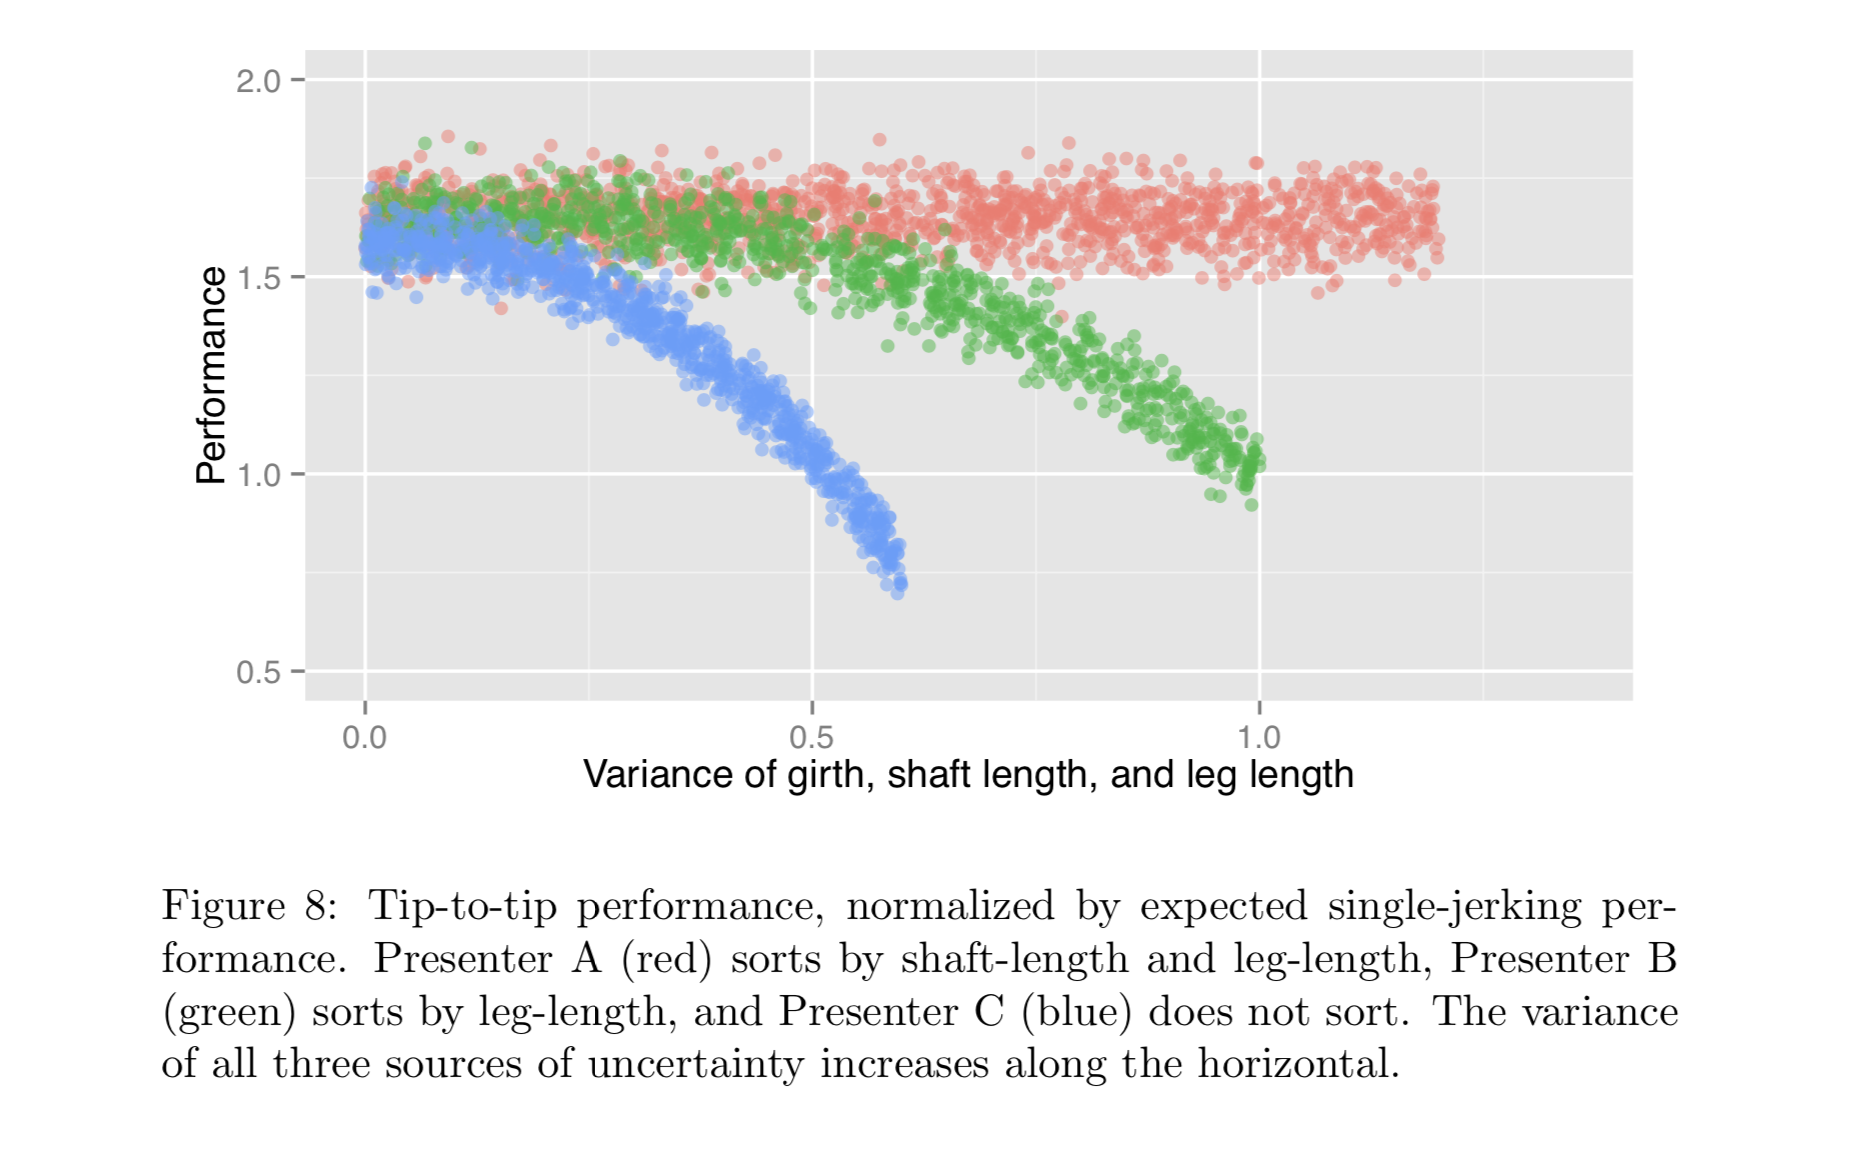
\includegraphics[width=9cm]{sorting}
    \end{figure}
\end{frame}


\end{document}

